%%%%%%%%%%%%%%%%%%%%%%%%%%%%%%%%%%%%%%%%%
% Ay 190 - WS2
% Written by Chatarin Wong-u-railertkun
%%%%%%%%%%%%%%%%%%%%%%%%%%%%%%%%%%%%%%%%%

%----------------------------------------------------------------------------------------
%	PACKAGES AND OTHER DOCUMENT CONFIGURATIONS
%----------------------------------------------------------------------------------------

\documentclass[11pt,letterpaper]{article}

% Load some basic packages that are useful to have
% and that should be part of any LaTeX installation.
%

\usepackage{graphicx}     % be able to include figures

\usepackage{xcolor}         % get nice colors

% change default font to Palatino (looks nicer!)
\usepackage[latin1]{inputenc}
\usepackage{mathpazo}
\usepackage[T1]{fontenc}

% load some useful math symbols/fonts
\usepackage{latexsym,amsfonts,amsmath,amssymb}
\usepackage{subcaption}

% comfort package to easily set margins
\usepackage[top=1in, bottom=1in, left=1in, right=1in]{geometry}

% control some spacings
%
% spacing after a paragraph
\setlength{\parskip}{.15cm}
% indentation at the top of a new paragraph
\setlength{\parindent}{0.0cm}

\usepackage{courier}

%----------------------------------------------------------------------------------------
%	TITLE
%----------------------------------------------------------------------------------------

\begin{document}

\begin{center}
\Large
Ay190 -- Worksheet 02 \\    %%%%%% DON'T FORGET TO CHANGE THE WORK SHEET NUMBER
Chatarin (Mee) Wong-u-railertkun\\
Date: \today
\end{center}

%----------------------------------------------------------------------------------------
%	QUESTION 1
%----------------------------------------------------------------------------------------

\section{An Unstable Calculation}
Create a python function to calculate sequence and recurrence relation described in the problem, called
\texttt{\bf recur13}, in the file \texttt{Ay190\_Lib\_2.py}

\begin{table}[h]
	\centering
	\begin{tabular}{r | r | r | r | r}
		% Table Header
		n & Recur Value & Closed form Value & Absolute Error & Relative Error \\
		\hline
		\hline
		% table data
		0 & 1.0 & 1.0 & 0.0 & 0.0 \\
		1 & 0.333333 & 0.333333 & 0.0 & 0.0 \\
		2 & 0.111111 & 0.111111 & -4.47035e-08 & -4.02331e-07 \\
		3 & 0.0370372 & 0.037037 & -1.82539e-07 & -4.92856e-06 \\
		4 & 0.0123464 & 0.0123457 & -7.31088e-07 & -5.92181e-05 \\
		5 & 0.00411815 & 0.00411523 & -2.92482e-06 & -0.000710731 \\
		6 & 0.00138344 & 0.00137174 & -1.16988e-05 & -0.00852843 \\
		7 & 0.000504043 & 0.000457247 & -4.67952e-05 & -0.102341 \\
		8 & 0.000339597 & 0.000152416 & -0.000187181 & -1.22809 \\
		9 & 0.000799529 & 5.08053e-05 & -0.000748724 & -14.7371 \\
		10 & 0.00301183 & 1.69351e-05 & -0.00299489 & -176.846 \\
		11 & 0.0119852 & 5.64503e-06 & -0.0119796 & -2122.15 \\
		12 & 0.0479202 & 1.88168e-06 & -0.0479183 & -25465.8 \\
		13 & 0.191674 & 6.27225e-07 & -0.191673 & -305589.0 \\
		14 & 0.766693 & 2.09075e-07 & -0.766693 & -3.66707e+06 \\
		15 & 3.06677 & 6.96917e-08 & -3.06677 & -4.40048e+07 \\
		\hline
	\end{tabular}
	\caption{Table shows values from recurring method, and closed form, including absolute and relative errors for n = 0, 1, 2, ..., 15.
	Numbers are shown with single digit precision FP numbers.}
	\label{tab:Recurring}
\end{table}

Thus, even at such a low \emph{n} as 15, the relative error grows up to $10^7$ already.

%----------------------------------------------------------------------------------------
%	QUESTION 2
%----------------------------------------------------------------------------------------

\section{Finite Difference Approximation and Convergence}
Create a python function to calculate first-order derivative using forward differencing and central differencing, called
\texttt{\bf forward} and \texttt{\bf central}, in the file \texttt{Ay190\_Lib\_2.py}, respectively.

It turns out that even at step size $h=10^{-3}$, the differences between these two methods are hard to notice when plotted against each other.
Thus, in figure \ref{fig:DiffMethod}, I plot with $h=1$ to intentionally exaggerate the error. Moreover, I plot the analytical answer for the first
order derivative of the function.

\begin{figure}[h!]
	\centering
	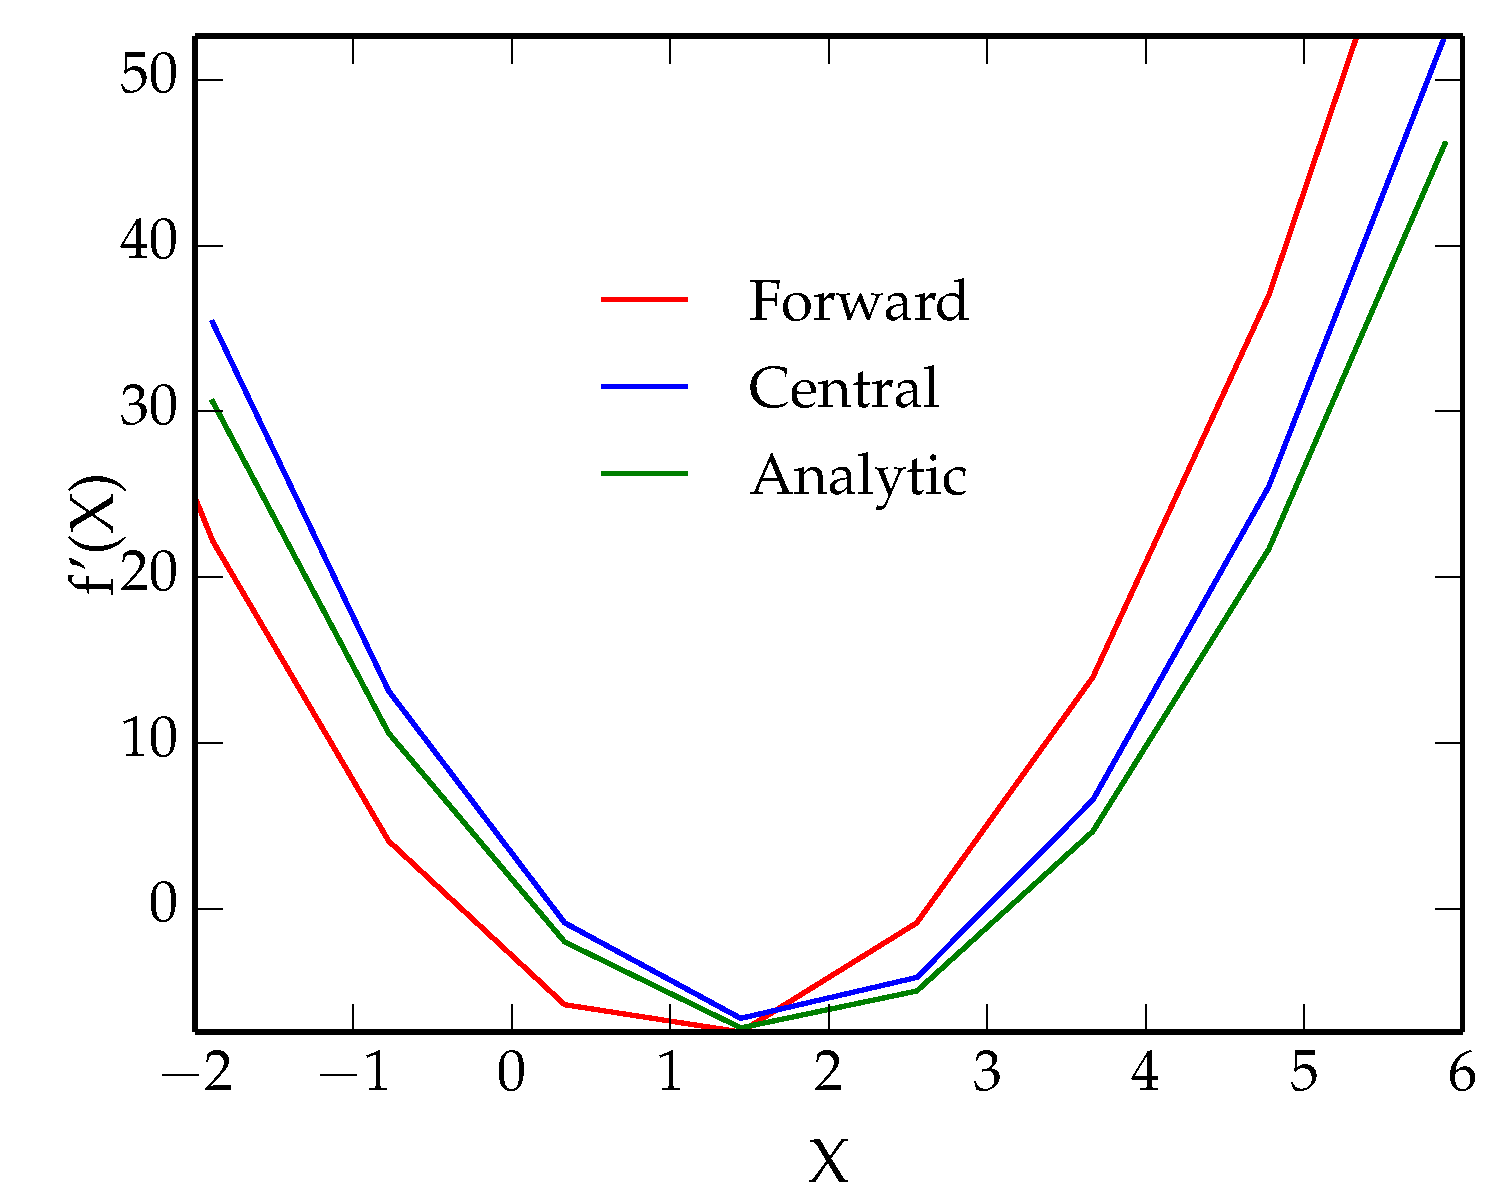
\includegraphics[width=0.5\textwidth]{CompareMethods}
	\caption{Comparing answer from two different methods in finding first-order derivative, against the analytical answer. The step size is 1, 
	to exaggerate the error.}
	\label{fig:DiffMethod}
\end{figure}

Figure \ref{fig:ForwardErr} and figure \ref{fig:CentralErr} illustrate the convergence rate of forward and central differencing, respectively.
We can see that the absolute error for forward differencing method is reduced linearly with step size $h$ as expected. However, the absolute
error for the central differencing method doesn't go down quadratically as expected.

\begin{figure}[h!]
	\centering
	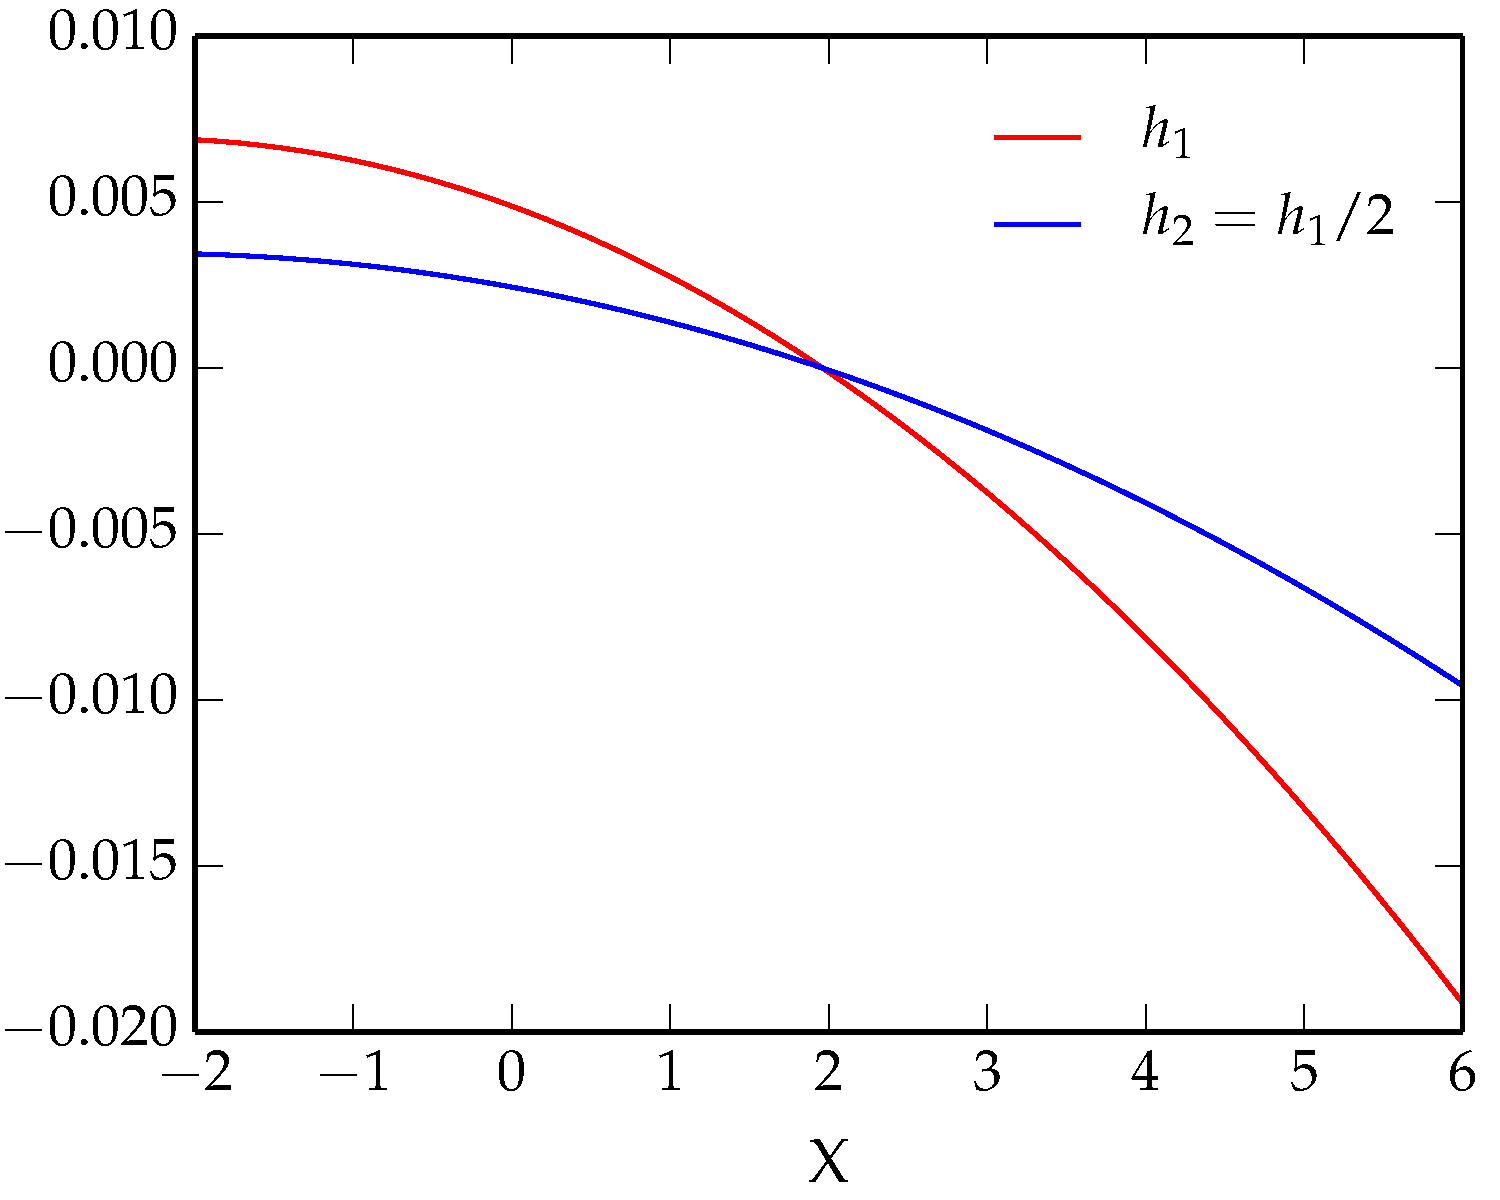
\includegraphics[width=0.5\textwidth]{ForwardErr}
	\caption{Showing absolute errors of forward differencing method with two different \emph{h}, with $h_1=10^{-3}$. We can see that the error reduce
	linearly with \emph{h} as expected.}
	\label{fig:ForwardErr}
\end{figure}

\begin{figure}[h!]
	\centering
	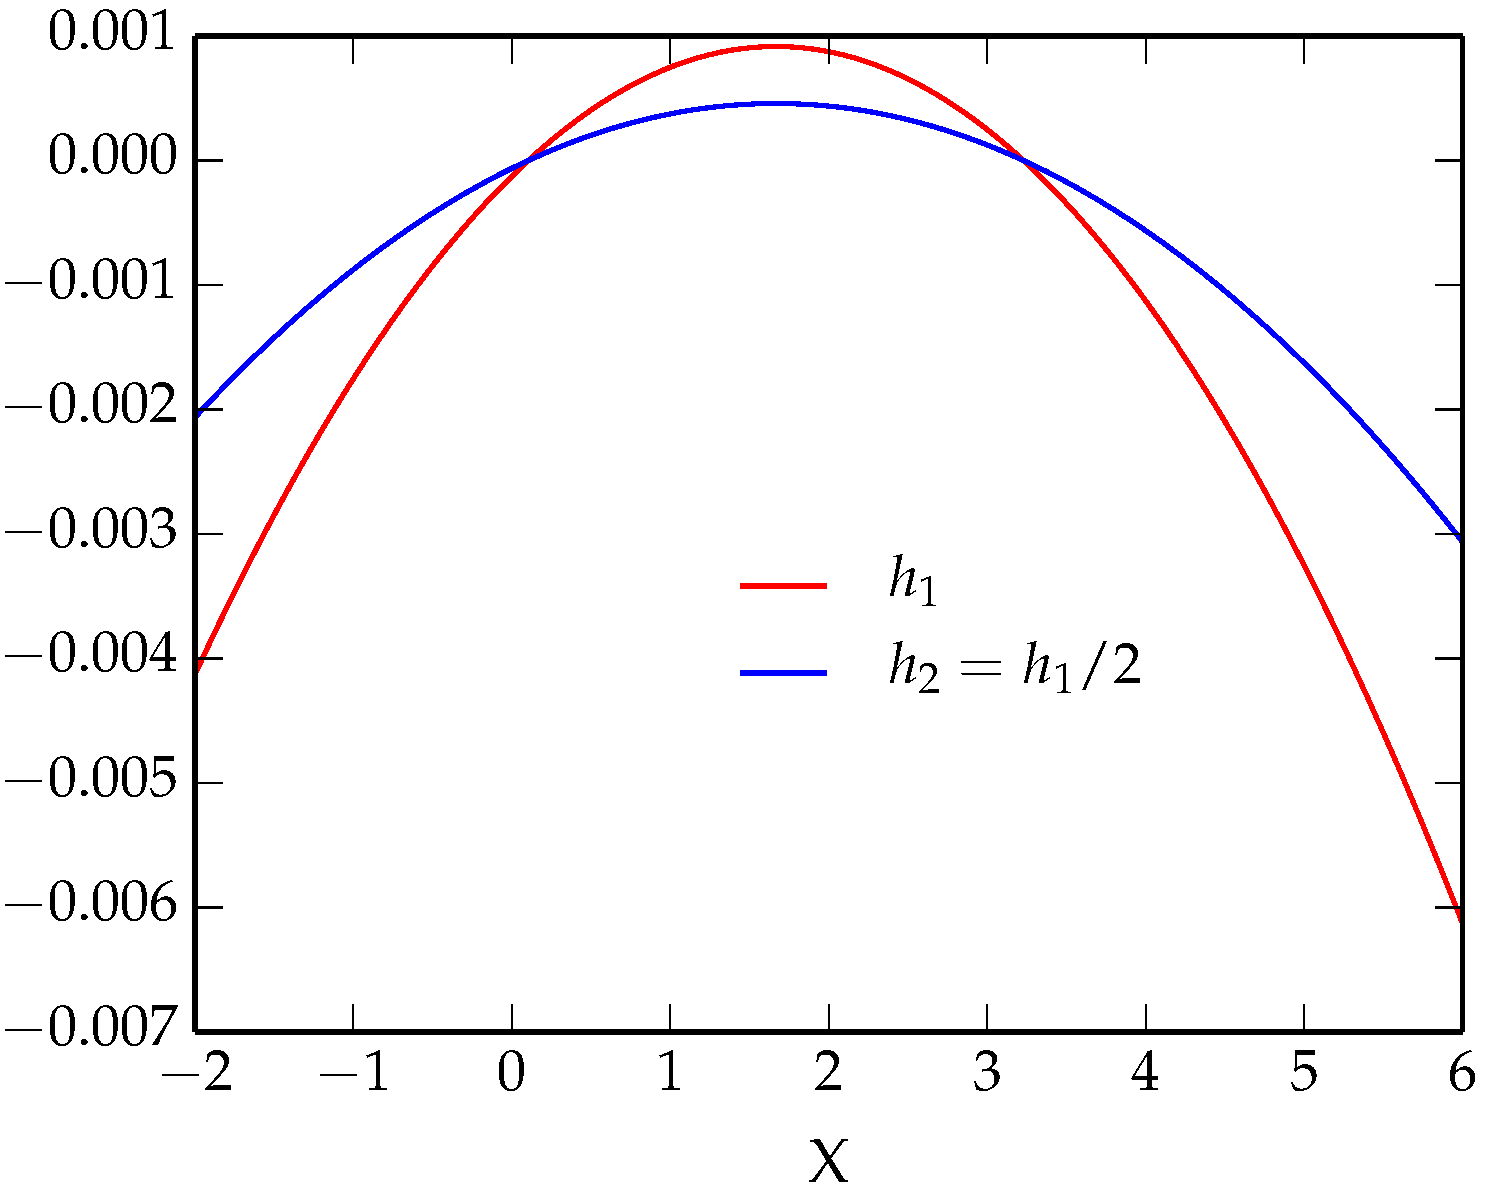
\includegraphics[width=0.5\textwidth]{CentralErr}
	\caption{Showing absolute errors of central differencing method with two different \emph{h}, with $h_1=10^{-3}$. However, the error reduce
	linearly with \emph{h}, instead of quadratically as expected.}
	\label{fig:CentralErr}
\end{figure}

%----------------------------------------------------------------------------------------
%	QUESTION 3
%----------------------------------------------------------------------------------------

\newpage

\section{Second Derivative}

Similar to in the class notes, we use Taylor's theorem to find an approximation for f' at $x_o$:

	\begin{align*}
	f(x_o+h) &= f(x_o)+hf'(x_o)+\frac{h^2}{2}f''(x_o) + \frac{h^3}{6}f'''(x_o) + O(h^4) \\
	f(x_o-h) &= f(x_o)-hf'(x_o)+\frac{h^2}{2}f''(x_o) - \frac{h^3}{6}f'''(x_o) + O(h^4)
	\end{align*}

Combine these two equations together

	\begin{equation}
	f(x_o+h)+f(x_o-h) = 2f(x_o) + h^2 f''(x_o) + O(h^4) \nonumber
	\end{equation}

Then, by solving for the second-order derivative

	\begin{equation}
	f''(x_o) = \frac{f(x_o+h)-2f(x_o)+f(x_o-h)}{h^2} + O(h^2) \nonumber
	\end{equation}

%----------------------------------------------------------------------------------------
%	QUESTION 4
%----------------------------------------------------------------------------------------

\section{Interpolation: Cepheid Lightcurve}

\subsection{Global Lagrange Interpolation}

Figure \ref{fig:GlobalLagrange} illustrates the global Lagrange interpolation against its 9 known data points.
We could see the Runge's phenomenon of non-convergence toward the boundary points.

\begin{figure}[h!]
	\centering
	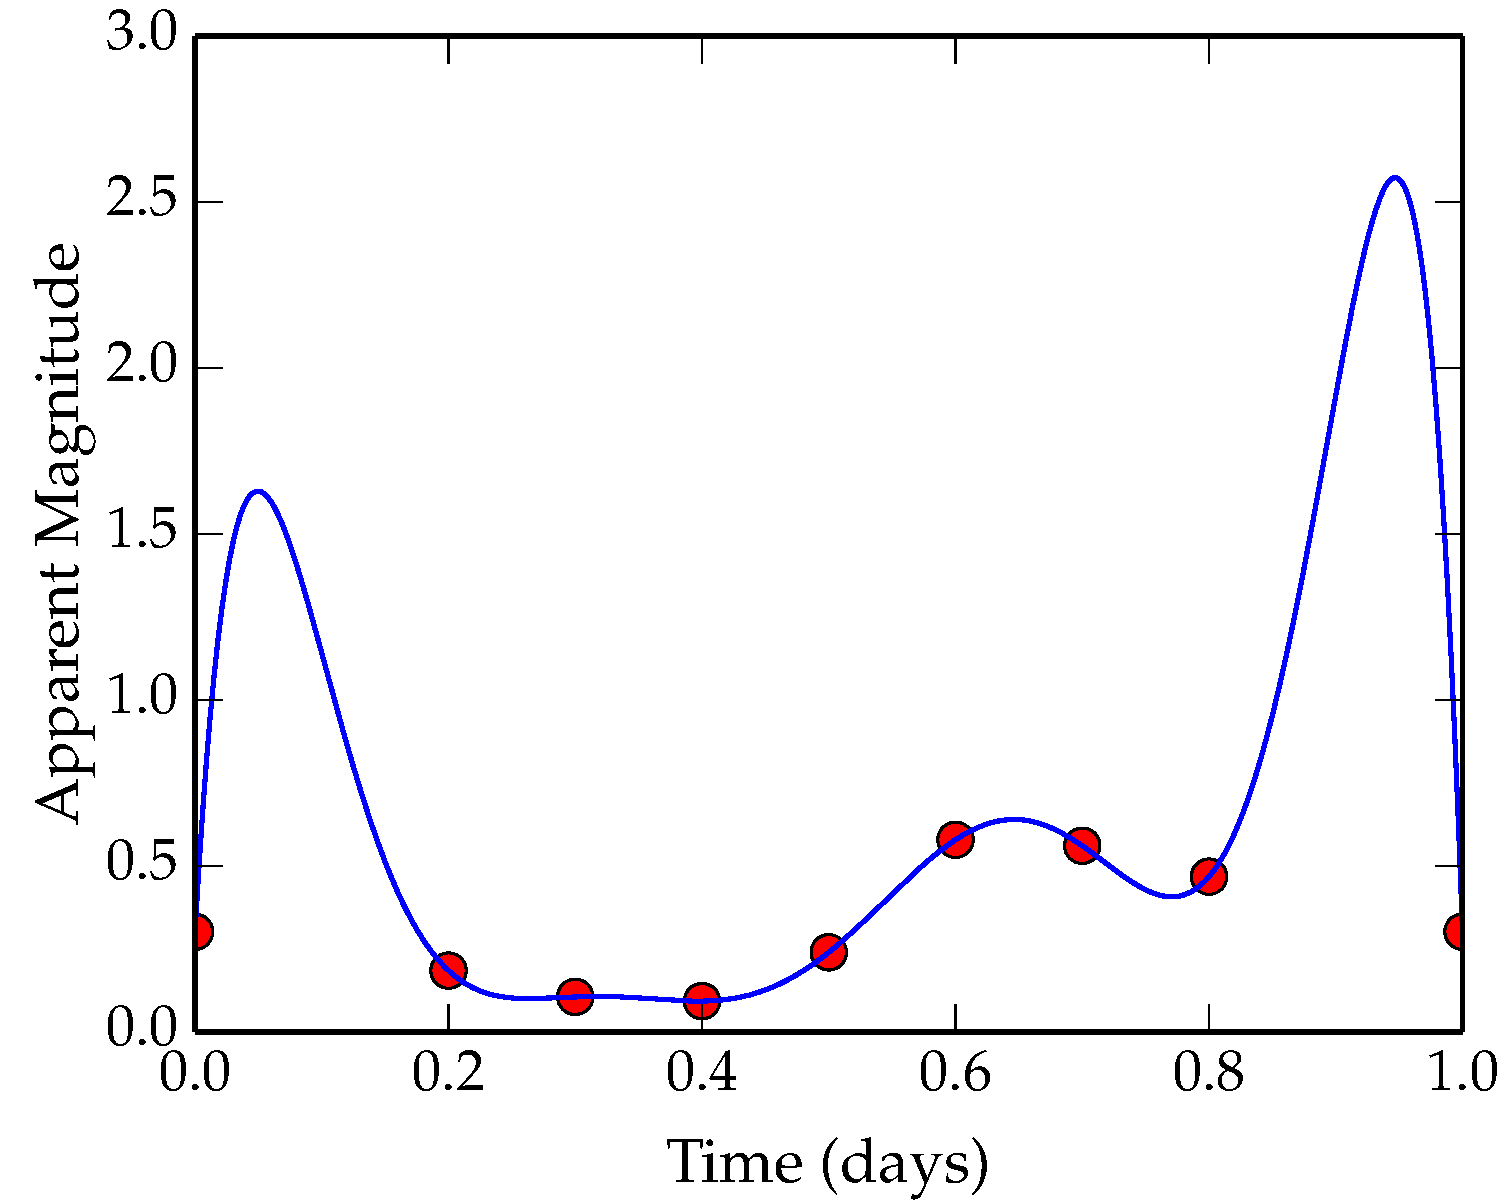
\includegraphics[width=0.5\textwidth]{GlobalLagrange}
	\caption{Plotting a single global Lagrange interpolation polynomial against its 9 known data points.}
	\label{fig:GlobalLagrange}
\end{figure}

\subsection{Linear Vs. Quadratic Interpolation}

Figure \ref{fig:DiffInter} compares results from linear and quadratic interpolation of the same data.

\begin{figure}[h!]
	\centering
	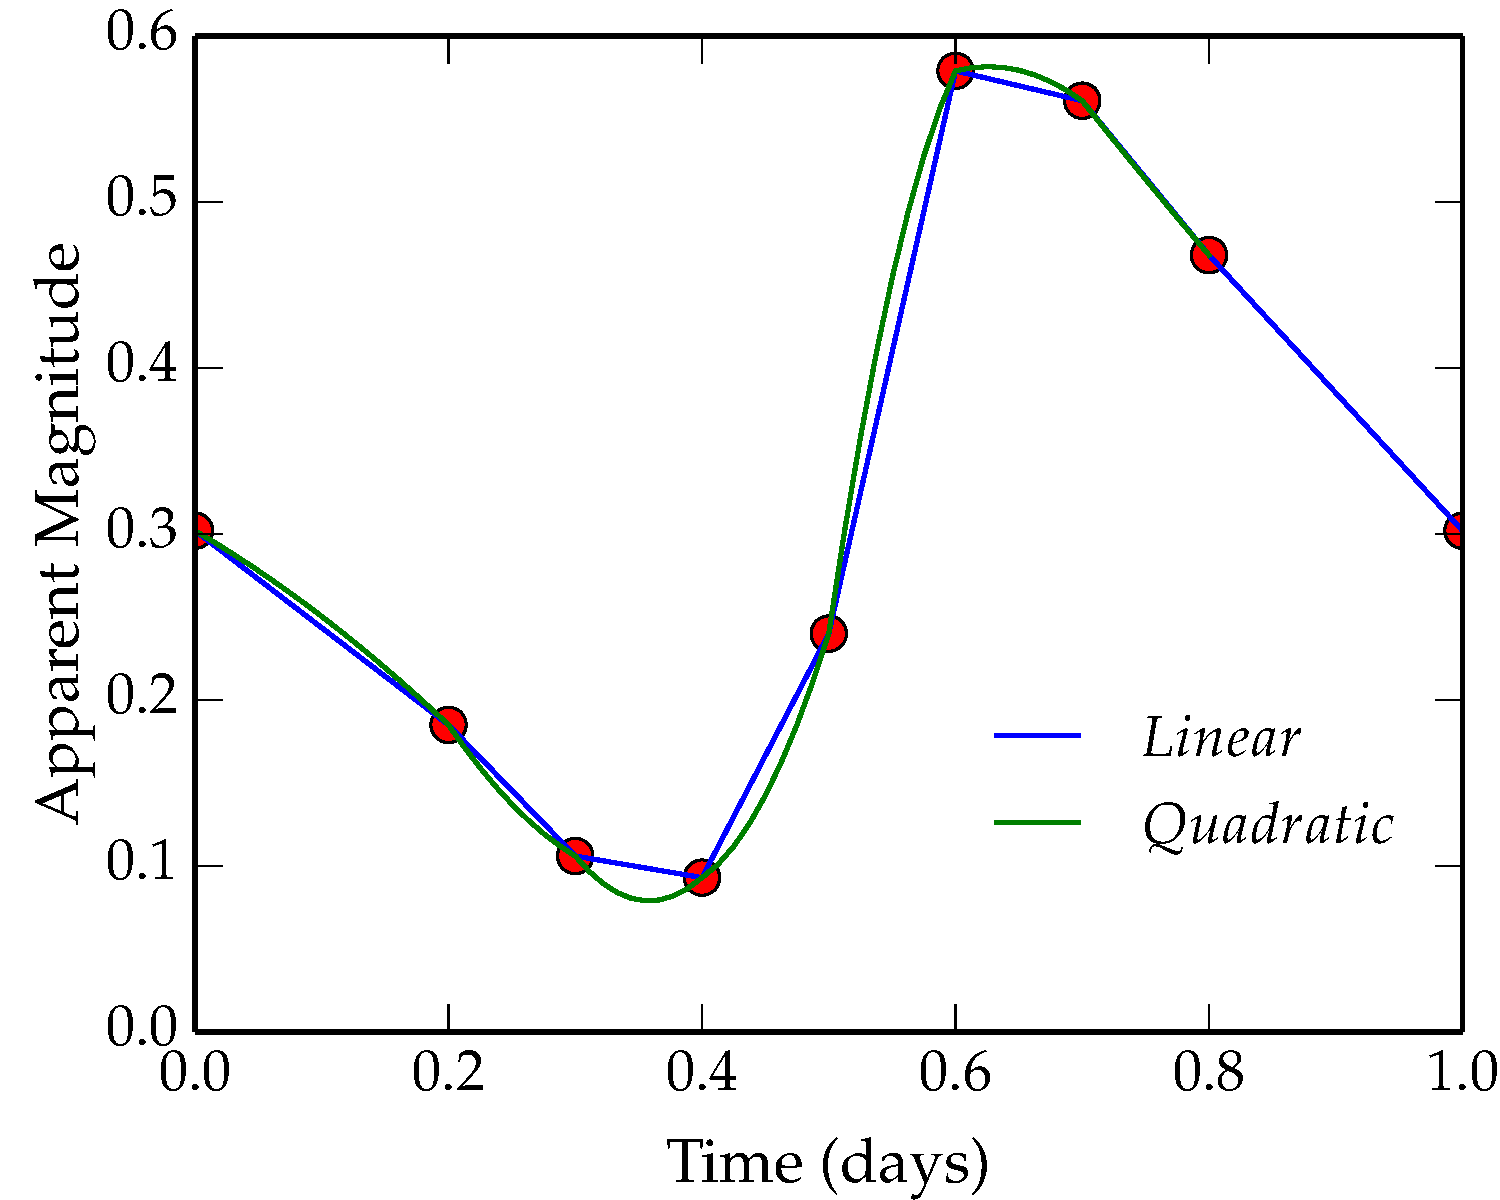
\includegraphics[width=0.5\textwidth]{DiffInter}
	\caption{Comparing results from two different methods, linear and quadratic interpolation, on the same set of data}
	\label{fig:DiffInter}
\end{figure}

%----------------------------------------------------------------------------------------
%	QUESTION 5
%----------------------------------------------------------------------------------------

\section{More Cepheid Lightcurve Interpolation}

\subsection{Piecewise Cubic Hermite Interpolation}

\begin{figure}[h!]
	\centering
	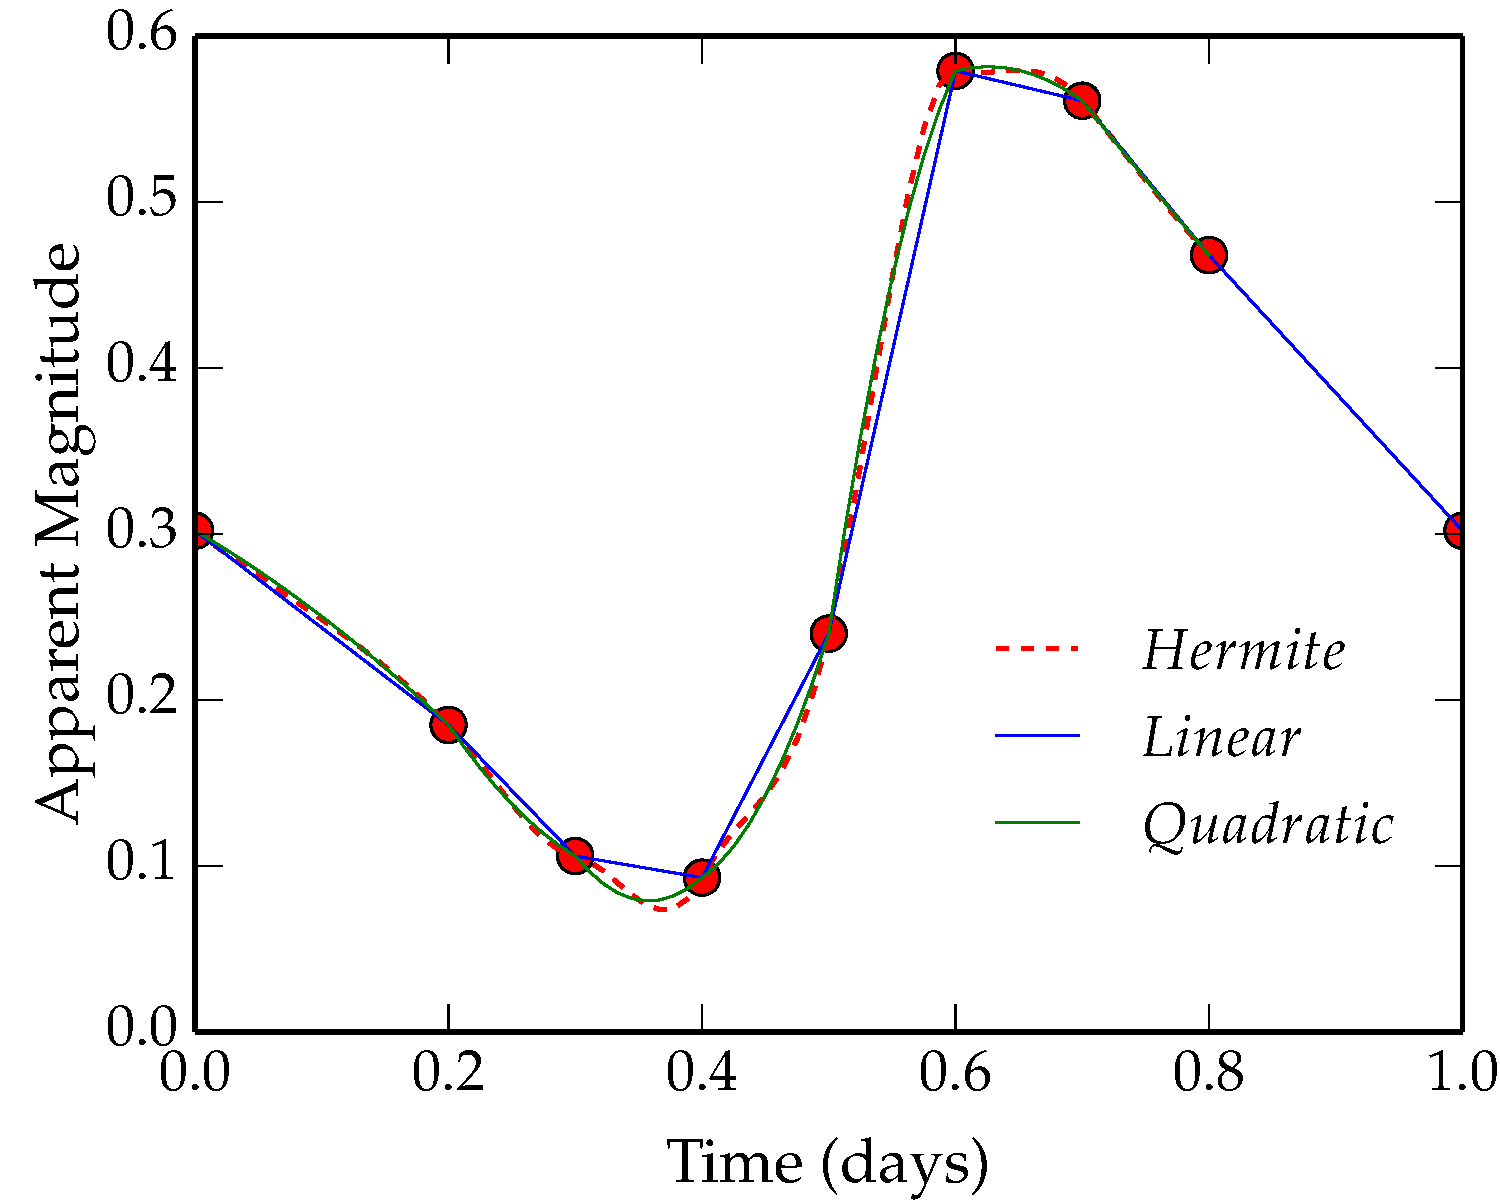
\includegraphics[width=0.5\textwidth]{HermiteInter}
	\caption{}
	\label{fig:HermiteInter}
\end{figure}

\subsection{Cubic Spline Interpolation}

Using Scipy.interpolate to perform cubic spline interpolation, instead of writing my own function.

\begin{figure}[h!]
	\centering
	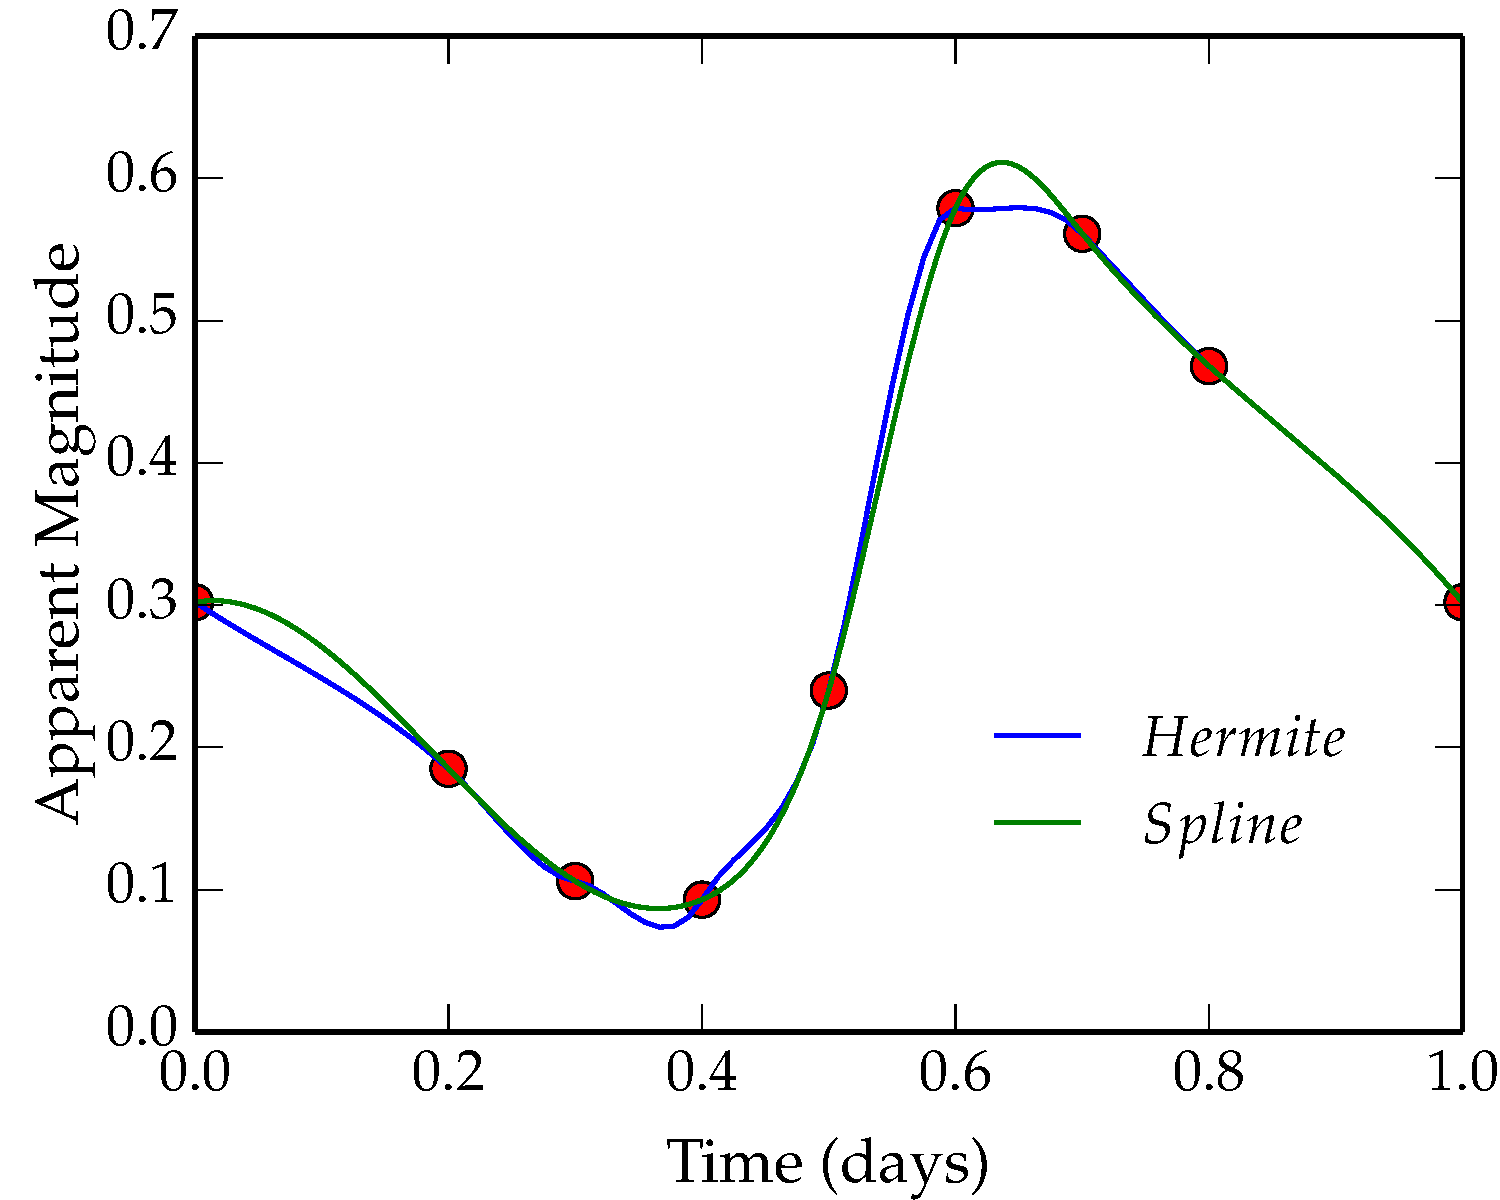
\includegraphics[width=0.5\textwidth]{SplineInter}
	\caption{}
	\label{fig:SpineInter}
\end{figure}

%----------------------------------------------------------------------------------------
%	NOTE
%----------------------------------------------------------------------------------------
 
 \section{Note}
 All python functions created are grouped together in the file \texttt{Ay190\_Lib\_2.py}. Other python scripts, used to create figures, are named in the
 format of Q[question number]-[order of figure in that question].py

\end{document}

